\subsubsection{Sprint goal}
Lo sprint è stato principalmente dedicato a studiare le API di Twitter e produrre le prime funzionalità per la visualizzazione e l'analisi dei tweet.\\
In particolare le feature pianificate per lo sprint sono state:
\begin{itemize}
    \item Ricerca di tweet per username
    \item Ricerca di tweet per hashtag
    \item Analisi dei tweet tramite componenti grafiche:
    \begin{itemize}
        \item Grafico a torta per il sentiment analysis
        \item Grafico a barre per la frequenza dei Tweet
        \item Word cloud con le parole più usate
    \end{itemize}
\end{itemize}


\subsubsection{Backlog}
\userstory%
{Come utente interessato ai tweet,\\voglio poter cercare dei tweet per hashtag\\per leggerli.}%
{8\\(3 frontend + 5 backend)}%
{L'utente, cercando un hashtag in un apposito textbox, è in grado di leggere tutti i tweet correlati visualizzando:
nome account Twitter, username, immagine profilo, contenuto tweet (testo + foto e video), data e ora, luogo (se applicabile), numero like, numero commenti, numero retweet.}%
{Richiamare l'API implementata, verificare che il formato sia corretto e che il contenuti dei tweet contenga l'hashtag ricercato.}
{Raccolta e analisi di tweet}

\userstory%
{Come utente interessato ai tweet,\\voglio poter cercare dei tweet per nome utente\\per leggerli.}%
{8\\(3 frontend + 5 backend)}%
{L'utente, cercando un nome utente in un apposito textbox, è in grado di leggere tutti i tweet correlati visualizzando:
nome account Twitter, username, immagine profilo, contenuto tweet (testo + foto e video), data e ora, luogo (se applicabile), numero like, numero commenti, numero retweet.}%
{Richiamare l'API implementata, verificare che il formato sia corretto e che l'autore dei tweet sia quello ricercato.}
{Raccolta e analisi di tweet}

\userstory%
{Come analista,\\voglio poter analizzare il sentimento\\per stabilire se un tweet è positivo o meno.}%
{9\\(2 frontend + 7 backend)}%
{L'utente, dato un tweet, vede se è positivo, negativo o neutro tramite immagine o testo.}%
{Analizzare frasi di cui è noto il sentimento.}
{Raccolta e analisi di tweet}

\userstory%
{Come analista,\\voglio vedere un grafico a barre\\per vedere il numero di tweet nell'unità di tempo.}%
{2\\(2 frontend)}%
{L'utente apre una pagina web contenente il grafico a barre con il numero di tweet nell'unità di tempo.}%
{Manualmente verificare che il grafico sia corretto.}
{Raccolta e analisi di tweet}

\userstory%
{Come analista,\\voglio vedere un grafico a torta\\per vedere il rapporto di sentiment positivi, negativi e neutri.}%
{2\\(2 frontend)}%
{L'utente apre una pagina web contenente il grafico a torta con sentiment positivi, negativi e neutri.}%
{Manualmente verificare che il grafico sia corretto.}
{Raccolta e analisi di tweet}

\userstory%
{Come analista,\\voglio vedere una term cloud\\per vedere le parole più utilizzate nei tweet.}%
{4\\(2 frontend + 2 backend)}%
{L'utente apre una pagina web contenente una term cloud con le parole più utilizzate.}%
{Manualmente verificare che il grafico sia corretto.}
{Raccolta e analisi di tweet}

\newpage
\subsubsection{Esito sprint}
Lo sprint è terminato con la conclusione di tutte le user stories pianificate.\\
Il lavoro è risultato omogeneo, con un piccolo scostamento rispetto all'andamento ideale 
che però non è stato causa di imprevisti o ritardi.\\
\begin{figure}[H]
    \centering
    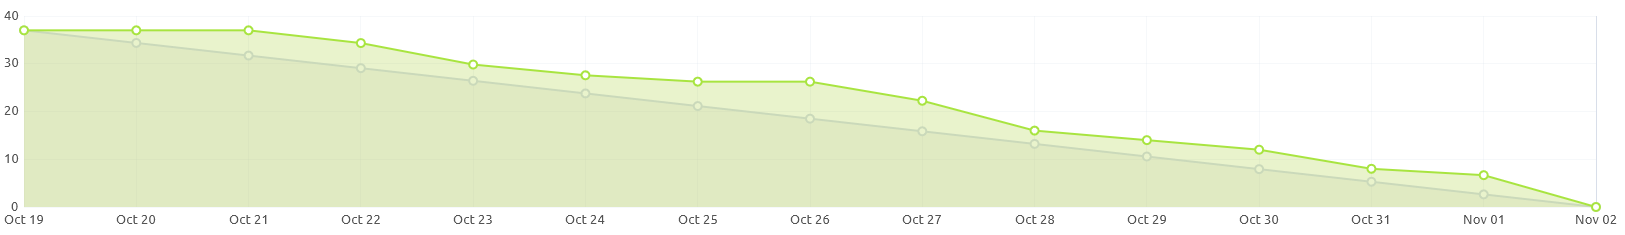
\includegraphics[width=15cm]{./img/sprint1/burndown.png}
    \caption{Burndown sprint 1}
\end{figure}
Anche le ore di lavoro (con il tempo stimato in quanto allo sprint 1 non è stato effettuato il monitoraggio) sono risultate in linea con il monte ore previsto.\\
\begin{figure}[H]
    \centering
    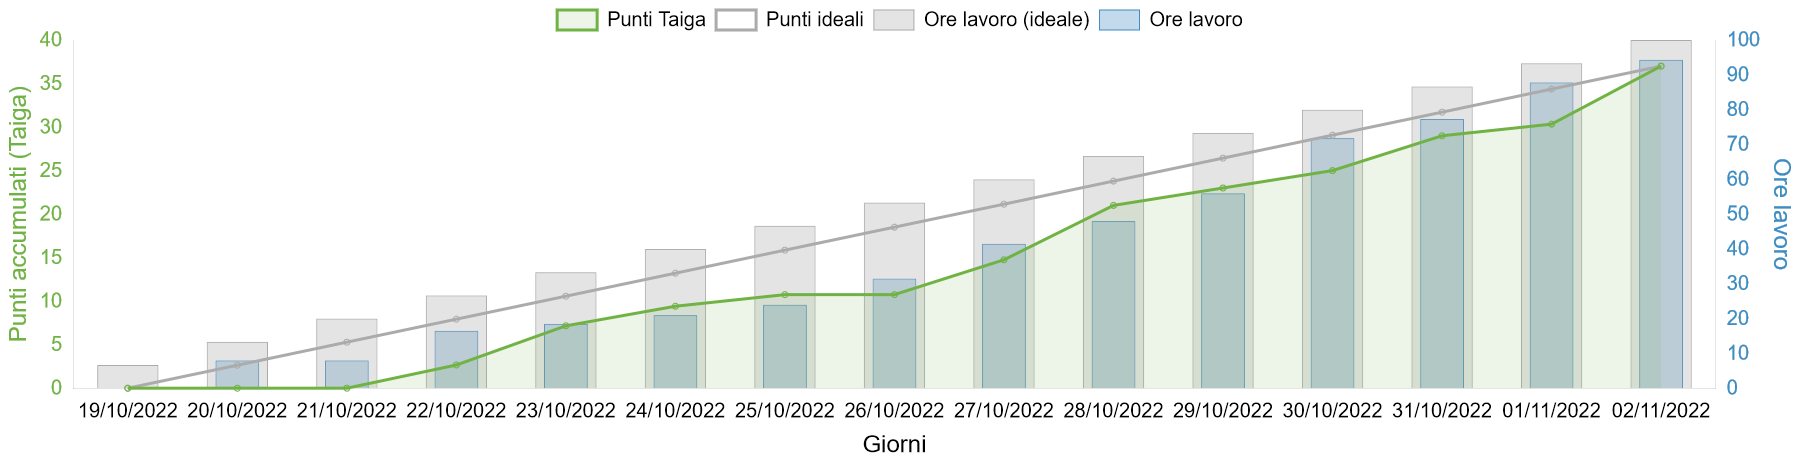
\includegraphics[width=15cm]{./img/sprint1/worktime.png}
    \caption{Progresso dei punti (asse a sinistra) e ore di lavoro (asse a destra)}
\end{figure}


\subsubsection{Sprint review}
Alla sprint review è stato chiesto dal cliente l'implementazione delle seguenti feature:
\begin{itemize}
    \item Ricerca di tweet per intervallo temporale
    \item Possibilità di selezionare il numero di tweet da estrare con una singola richiesta
\end{itemize}


\newpage
\subsubsection{Retrospettiva}
\subsubsection*{Pre-retrospettiva}
Alla pre-retrospettiva effettuata a metà sprint, sono emerse le seguenti problematiche:
\begin{itemize}
    \item Tempo dedicato al lavoro non sufficiente
    \item Mancanza di comunicazione nel team
    \item Task e user stories hanno descrizioni poco dettagliate e facilmente fraintendibili
\end{itemize}
\begin{figure}[H]
    \centering
    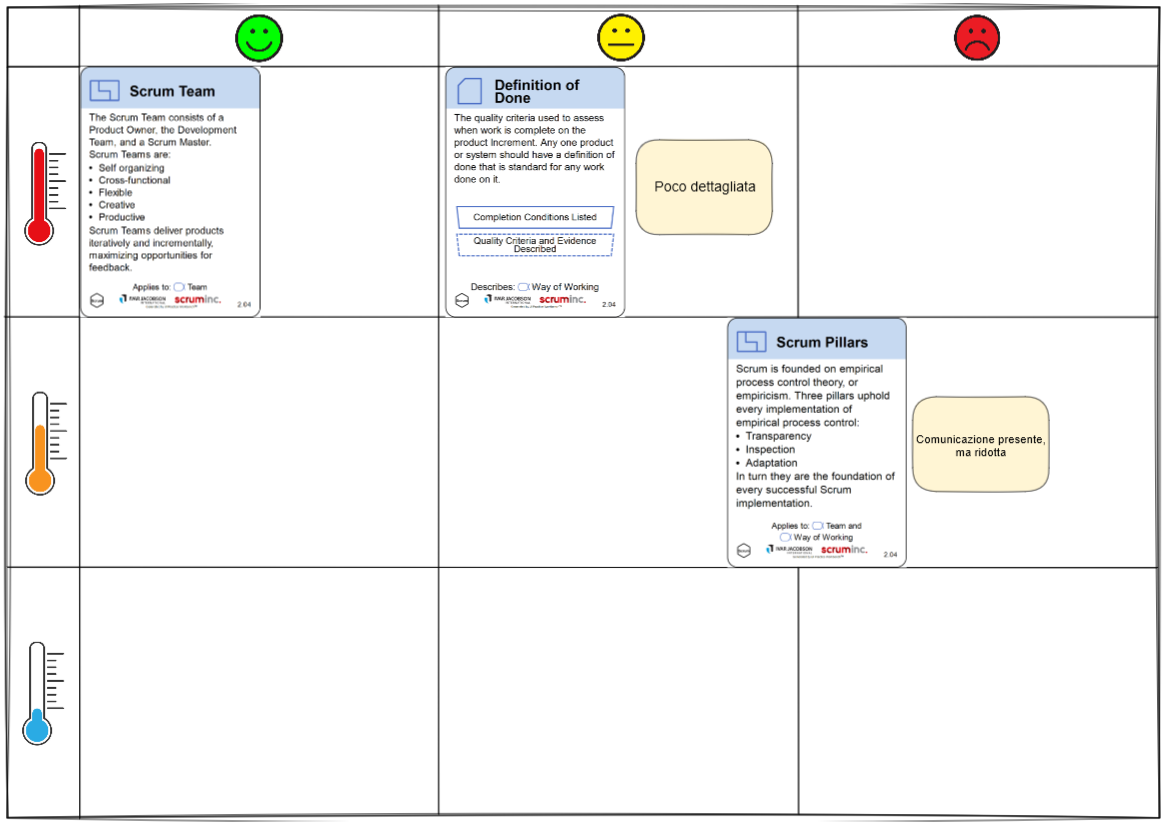
\includegraphics[width=15cm]{./img/sprint1/preretrospettiva.png}
    \caption{Pre-retrospettiva del 27/10/2022}
\end{figure}

\subsubsection*{Retrospettiva}
Alla retrospettiva di fine sprint, gli aspetti positivi evidenziati dal team sono:
\begin{itemize}
    \item Il deliverable presentato alla sprint review è risultato adeguato e funzionante
    \item Il team e i ruoli di ciascuno sono ben definiti
\end{itemize}
Sono invece stati portati all'attenzione del team i seguenti problemi:
\begin{itemize}
    \item Non è stato effettuato un monitoraggio delle ore di lavoro (che è stato quindi stimato sulla base sui daily scrum virtuali)
    \item I problemi evidenziali alla pre-retrospettiva non sono ancora stati risolti 
\end{itemize}
\begin{figure}[H]
    \centering
    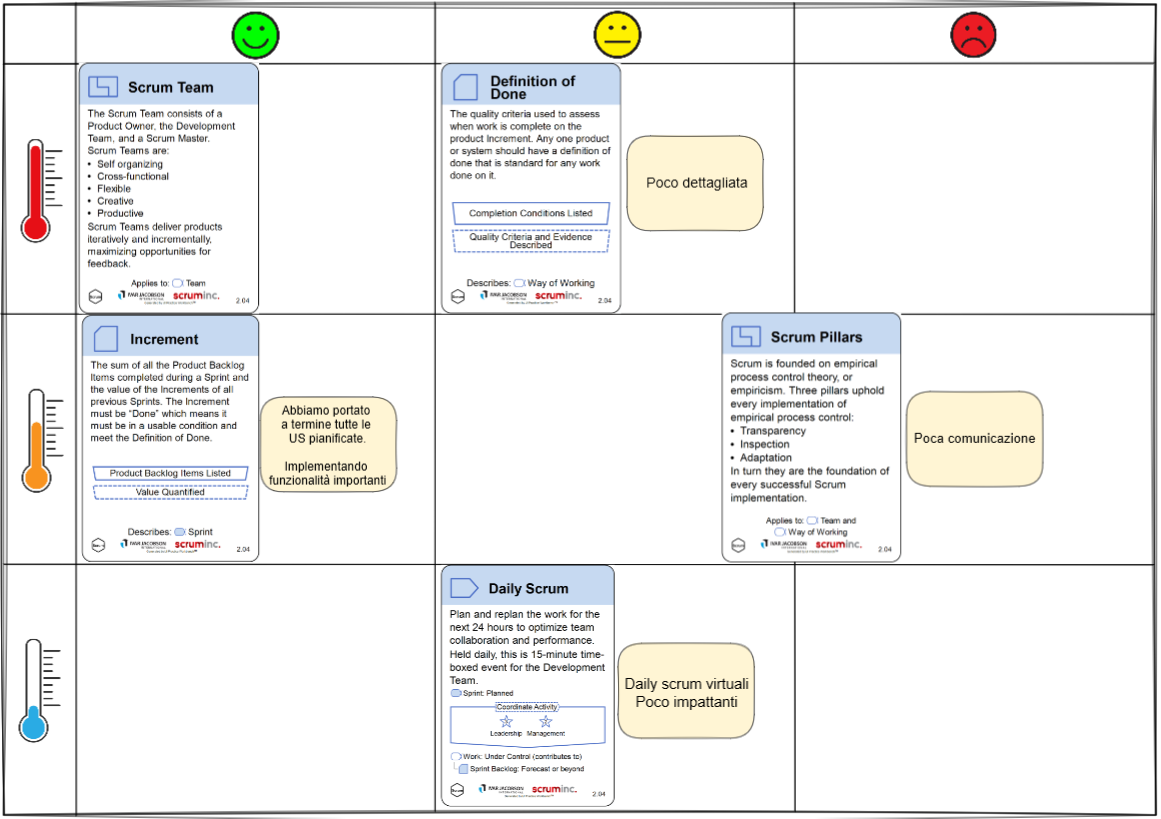
\includegraphics[width=15cm]{./img/sprint1/retrospettiva.png}
    \caption{Retrospettiva del 01/11/2022}
\end{figure}